\documentclass[../main/main.tex]{subfiles}
\graphicspath{{./figures/}}
\usepackage{pdfpages}

\makeatletter
\renewcommand{\@chapapp}{Travaux pratiques -- TP}
\makeatother

\toggletrue{student}
% \HideSolutionstrue
% \toggletrue{corrige}
% \renewcommand{\mycol}{black}
\renewcommand{\mycol}{gray}

\begin{document}
\setcounter{chapter}{16}

\chapter{\cswitch{Correction du TP}
  {\'Etude du pendule simple}}

\enonce{
	\begin{prgm}
		\begin{tcb}*(ror)"how"{Savoir-faire}
			\begin{itemize}
				\item Capacité numérique~: à l’aide d’un langage de programmation,
				      résoudre numériquement une équation différentielle du deuxième ordre
				      non-linéaire et faire apparaître l’effet des termes non- linéaires.
				\item Mettre en œuvre un protocole expérimental permettant d’étudier une
				      loi de force par exemple à l’aide d’un microcontrôleur.
			\end{itemize}
		\end{tcb}
	\end{prgm}
	\vspace{-10pt}
	\section{Objectifs}
	\begin{itemize}
		\item Étudier le mouvement du pendule simple, par acquisition
		      informatisée grâce à l'interface \texttt{Sysam}.
		\item Interroger la conservation de l'énergie mécanique.
		\item Mise en évidence de l'approximation de l'énergie potentielle par un
		      puits de potentiel harmonique.
		\item Vérifier l'isochronisme des petites oscillations.
	\end{itemize}

	\section{S'approprier}

	Pour \textsc{Galilée}, la période des oscillations d'un pendule simple devait
	être indépendante de l'amplitude desdites oscillations. Dans ses
	\textit{Dialogues} (1632), il écrit~: «~Chacune de ces oscillations se fait dans
	des temps égaux, tant celle de $90\degres$, que celle de $50\degres$, ou de
	$20\degres$, de $10\degres$, de $4\degres$.~»

	\medskip

	26 ans plus tard, \textsc{Huygens} affine ce propos dans \textit{Horlogium
		Oscillatorium} en notant que «~seules les oscillations de \textbf{faible
		amplitude} doivent être considérées comme isochrones, c'est-à-dire avoir une
	période indépendante de l'amplitude.~»
}

\section{Analyser}

\noindent
\begin{minipage}{0.64\linewidth}
	Soit une masse $m = \SI{190}{g}$ attachée à l'extrémité d'une tige en fibre
	de carbone (de faible masse, pouvant être considérée négligeable devant
	celle de $m$) de longueur $\ell = \SI{45}{cm}$ constante. Initialement, la
	masse $m$ est lâchée d'un angle $\tt_0$ sans vitesse initiale. On prend $g =
		\SI{9,8}{m.s^{-2}}$.
\end{minipage}
\hfill
\begin{minipage}{0.34\linewidth}
	\begin{center}
		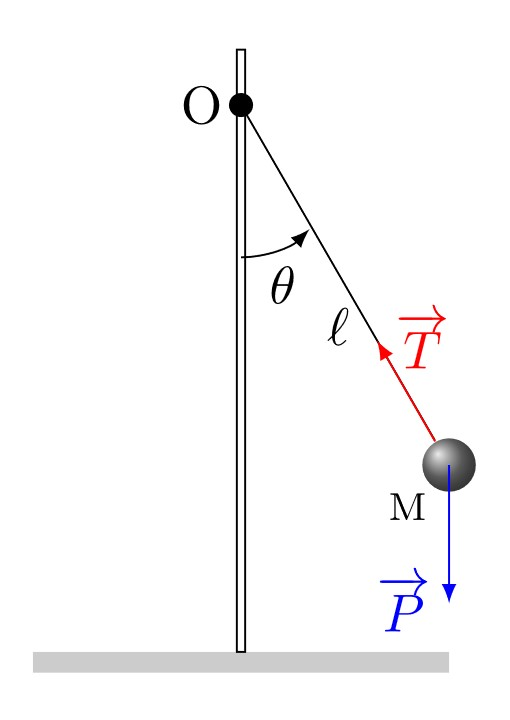
\includegraphics[width=3cm]{ch17pendule}
		% \captionof{figure}{Schéma du pendule simple.}
		% \label{fig:pendsimple}
	\end{center}
\end{minipage}
\setlist[blocQR,1]{leftmargin=10pt, label=\clenumi}
\QR{%
Montrer que l'énergie cinétique peut s'écrire sous la forme~:
\[
	\Ec_c = \frac{m\ell^2}{2}\tp^2
\]

}{%
On a un mouvement circulaire non uniforme, on trouve donc
\[
	\vf = \ell \tp \ut
	\Lra
	\Ec_c = \frac{1}{2}mv^{2}
	\Lra
	\boxed{\Ec_c = \frac{1}{2}m \ell^{2}\tp^{2}}
	\qed
\]
}
\QR{%
	En prenant l'origine des énergies potentielles en $\tt = 0$,
	montrer que l'énergie potentielle totale du système peut s'écrire
	sous la forme~:
	\[
		\Ec_{p,p} = mg\ell (1-\cos\tt)
	\]
}{%
	L'énergie potentielle de pesanteur s'écrit
	\[
		\Ec_{p,p} = mgz(\tt)
	\]
	Or, par rapport à la position $\tt = 0$ où le pendule est à la distance $\ell$
	du point O, à un angle $\tt$ quelconque la masse est à la distance $\ell\cos(\theta)$. On trouve donc
	\[
		z(\tt) = \ell(1-\cos(\theta))
		\Ra
		\boxed{\Ec_{p,p} = mg \ell(1-\cos(\theta))}
		\qed
	\]
}
\section{Réaliser}

\begin{tcb}[bld, cnt](impo){Important}
	Attention, la tige du pendule est en fibre de carbone et est TRÈS FRAGILE~;
	Ne pas serrer la vis de la masse trop fort sur la tige.
\end{tcb}

\begin{tcb}[breakable](expe)<itc>{Réglages}
	\begin{enumerate}
		\item Ouvrir le logiciel \texttt{Latispro}.
		\item Régler les paramètres d'acquisition~:
		      
\includegraphics[width=0.05\textwidth]{bouton1} $200$ points de mesure.
	\end{enumerate}
	\QR{%
		Indiquer le temps total d'acquisition $T\ind{acq,tot}$ permettant d'avoir
		quelques oscillations visibles.
		\smallbreak
		Que valent alors la durée d'échantillonnage $\Delta{t\ind{ech}}$ et la
		fréquence d'échantillonnage $\Delta{f\ind{ech}}$ de l'acquisition~? Vous
		expliquerez avec un schéma détaillé votre raisonnement.
	}{%
		On sait que la période est d'environ
		\[
			T_0 = 2\pi \sqrt{\frac{\ell}{g}}
			\qav
			\left\{
			\begin{array}{rcl}
				g    & = & \SI{9.81}{m.s^{-2}}
				\\
				\ell & = & \SI{45e-2}{m}
			\end{array}
			\right.\\
			\AN
			\xul{
				T_0 = \SI{1.35}{s}
			}
		\]
		Pour 4 périodes, il nous faut donc environ
		\[
			\xul{T\ind{acq,tot} \approx \SI{5.40}{s}}
		\]
		Avec $N = \num{200}$ points au total, on a une durée d'échantillonnage
		\[
			\Delta{t\ind{ech}} = \frac{T\ind{acq,tot}}{N} \approx \SI{2.7e-2}{s}
			\qor
			\boxed{f\ind{ech} = \frac{1}{\Delta{t\ind{ech}}}}
			\Lra
			\xul{f\ind{ech} = \SI{37}{Hz}}
		\]
	}
	\begin{enumerate}[resume]
		\item Faire le zéro de l'oscillateur en appuyant sur le petit bouton à
		      l'extrémité du fil noir près de la poulie, lorsque celui-ci est en
		      position verticale.
	\end{enumerate}
\end{tcb}

\begin{tcb}(expe)<itc>{Acquisition et enregistrement}
	\begin{enumerate}
		\item Écarter le pendule d'un angle de $\ang{20;;}$ à $\ang{30;;}$ environ.
		\item Lancer l'acquisition~: 
\includegraphics[width=0.03\textwidth]{bouton2}
	\end{enumerate}
\end{tcb}

\section{Valider}

\subsection{Exploitation de l'enregistrement}

\begin{tcb}(expe)<itc>{Visualisation des angles,
			vitesses et accélérations en fonction du temps}
	\begin{enumerate}
		\item En utilisant la feuille de calcul, créer une nouvelle variable, notée
		      \texttt{angle}, correspondant à l'angle exprimé en radians.
		\item Visualiser \texttt{angle} en fonction du temps~; ajuster l'échelle
		      grâce au calibrage (en cliquant droit).
		\item Créer les variables \texttt{deriv\_Pendule} (dérivée première) et
		      \texttt{dderiv\_Pendule} (dérivée seconde), en utilisant les fonctions
		      traitements $\rightarrow$ calculs spécifiques $\rightarrow$ dérivée et
		      dérivée seconde.
		\item À partir des variables \texttt{deriv\_Pendule} et
		      \texttt{dderiv\_Pendule} (exprimées en degrés), introduire les variables
		      \texttt{deriv\_angle} et \texttt{dderiv\_angle} exprimées en radians.
		\item Afficher simultanément les trois courbes obtenues et les lisser en
		      utilisant les fonctions traitements $\rightarrow$ calculs spécifiques
		      $\rightarrow$ lissage.
	\end{enumerate}
\end{tcb}

\setlist[blocQR,1]{leftmargin=10pt, label=\sqenumi}
\QR{%
	Imprimer vos courbes.
}{%
	Non corrigé.
}

\QR{%
	Déterminer et commenter les déphasages entre les différentes courbes.
	Justifier mathématiquement ces déphasages.
}{%
	On trouve
	\[
		\Delta{\f_{v/p}} = -\frac{\pi}{2}
		\qqet
		\Delta{\f_{a/v}} = -\frac{\pi}{2}
	\]
	C'est logique, la vitesse est la dérivée de la position qui s'exprime comme
	un oscillateur harmonique en
	\[
		\tt(t) = \tt_0 \cos(\w_0t)
		\Ra
		\tp(t) = \w_0\tt_0 \cos(\w_0t-\frac{\pi}{2})
	\]
	Et de même pour l'accélération qui est la dérivée de la vitesse.
}

\subsubsection{Propriété de l'énergie mécanique}

\setlist[blocQR,1]{leftmargin=10pt, label=\clenumi}
\QR<[start=4]>{%
	Proposer une exploitation graphique permettant de visualiser
	graphiquement et simultanément la conservation de l'énergie mécanique
	ainsi que les échanges énergétiques entre énergie cinétique et énergie
	potentielle. Vous représenterez sur un même graphique $\Ec_p(t)$,
	$\Ec_c(t)$ et $\Ec_m(t)$.
}{%
	Grâce à la feuille de calculs, on détermine \texttt{Ec} et \texttt{Ep} les
	énergies cinétique et potentielle dont les expressions ont été démontrées dans
	la Partie~III, puis \texttt{Em = Ec + Ep} l'énergie totale.
	\smallbreak
	Pour observer la conservation de l'énergie, on doit observer l'éventuelle
	pente négative de \texttt{Em} en fonction du temps. Pour une durée
	d'expérience relativement courte, on a en effet ce constat~; plus longtemps et
	les frottements solides et visqueux diminuent l'énergie du pendule.
}

\setlist[blocQR,1]{leftmargin=10pt, label=\sqenumi}
\QR<[start=3]>{%
	Imprimer les courbes et les commenter.
}{%
	Non corrigé.
}

\subsubsection{Approximation harmonique autour de la position d'équilibre}

\setlist[blocQR,1]{leftmargin=10pt, label=\clenumi}
\QR<[start=5]>{%
	Proposer une exploitation permettant de vérifier la parabolisation
	(énergie potentielle est équivalente à un polynôme d'ordre 2 en $\tt$)
	de l'énergie potentielle autour de la position d'équilibre.
}{%
	On trace $\Ec_{p,p}(\tt)$ en mettant l'angle $\tt$ en abscisse et \texttt{Ep}
	en ordonnée sur \texttt{LatisPro}. On regarde visuellement que c'est une
	parabole, et on peut modéliser la courbe grâce à l'outil de modélisation.
}

\setlist[blocQR,1]{leftmargin=10pt, label=\sqenumi}
\QR<[start=4]>{%
	Réaliser l'exploitation proposée. Imprimer et commenter. Faire le
	développement limité autour de $\tt=0$ (position d'équilibre) de l'expression
	de l'énergie potentielle précédemment obtenue pour comparer à la valeur
	obtenue à l'aide d'un écart normalisé.
}{%
	Impression non corrigée. Ça marche. En effectuant le DL de $\cos(\theta)$ à
	l'ordre 2, on obtient
	\[
		\cos(\theta) \Sim_{\tt \to 0} 1 - \frac{\tt^{2}}{2}
		\Lra
		\Ec_{p,p}(\tt) = mg \ell(1 - \left( 1 - \frac{\tt^{2}}{2} \right))
		\Lra
		\boxed{\Ec_{p,p}(\tt) = \frac{1}{2}mg \ell \tt^{2}}
	\]
	On doit trouver que le coefficient directeur de la modélisation est égal à
	\begin{gather*}
		\boxed{a = \frac{1}{2}m \ell^{2}}
		\qav
		\left\{
		\begin{array}{rcl}
			m    & = & \SI{190e-3}{kg}
			\\
			\ell & = & \SI{45e-2}{m}
		\end{array}
		\right.\\
		\AN
		\xul{
			a\ind{theo} \approx \SI{1.9e-2}{J}
		}
	\end{gather*}
	Expérimentalement, on trouve
	\[
		a\ind{exp} = \SI{1.9\pm0.1e-2}{J}
	\]
	D'où l'écart
	\[
		E_N = \frac{\abs{a\ind{exp} - a\ind{theo}}}{u(a\ind{exp})}
		\Lra
		\xul{E_N = ?}
	\]
	Malgré les frottements, on trouve une réponse similaire, ce qui valide le
	faible angle.
}

\subsection{Amplitude et (non-)isochronisme des oscillations}

\subsubsection{Protocole expérimental}

\QR{%
	Proposer puis réaliser un protocole expérimental qui permettrait de
	lever la contradiction historique présentée dans la partie S'approprier,
	sans dépasser un angle initial de $60\degres$ environ (on pourra
	utiliser l'icône~: Outils $\rightarrow$ mesures automatiques).
}{%
	Pour plusieurs valeurs de $\tt_0$, on mesure la période $T$ observée grâce aux
	curseurs de \texttt{LatisPro}. On remplit un tableau de valeurs et on compare
	cette période à la période des petites oscillations $T_0 = 2\pi
		\sqrt{\frac{\ell}{g}}$.
}

\QR{%
	Présenter vos mesures sous forme d'un tableau $T\ind{exp} = f(\tt_0)$
	et d'une courbe expérimentale que vous imprimerez et commenterez.
	Conclure quant à l'isochronisme (ou non) des oscillations.
}{%
	Il n'y a pas d'isochronisme, $T \neq T_0$ à partir de $\tt_0 \approx
		\ang{40}$.
}

\QR{%
	En déduire la valeur de $T\ind{iso}$ en tenant compte de vos
	différents mesurages \textbf{dans le cas où il y a isochronisme}.
	Comparer avec $T_0$ la période propre du pendule pour les petits angles
	par un écart normalisé.
}{%
	C'est la valeur la plus basse du tableau. On trouve…
}

\subsubsection{Résolution numérique}

L'objectif de cette résolution numérique est de résoudre l'équation
différentielle non linéarisée et donc non analytique~:
\[
	\tpp + {\w_0}^2 \sin(\tt) = 0
\]

\setlist[blocQR,1]{leftmargin=10pt, label=\clenumi}
\QR<[start=6]>{%
	Dans un premier temps, vous allez compléter le script suivant sur
	\texttt{Capytale} à ce lien~:
	\url{https://capytale2.ac-paris.fr/web/c/eb53-1348043}. Il devra
	permettre de résoudre, pour une condition initiale $\tt_0$ donnée,
	l'équation différentielle ci-dessus à l'aide du schéma numérique python
	\texttt{solve\_ivp}. Pour ce faire, vous devrez importer
	\texttt{scipy.integrate} au début de votre script avec
	\begin{center}
		\texttt{from scipy.integrate import solve\_ivp}
	\end{center}
	Pour vous aider, consulter la page suivante~:
	\url{https://tinyurl.com/pythonsolveivp}.
}{%
	Voir corrigé~: \url{https://capytale2.ac-paris.fr/web/c/21b7-2947279}
}
Le script précédent sera ensuite amélioré afin de résoudre l'équation
différentielle pour un ensemble de solutions initiales comprises entre
$\tt_0 \approx 0$ et $\tt_0 = \pi/2$. Vous trouverez la fréquence de
chaque solution grâce à une fonction \texttt{freqfinder} déjà créée
l'occasion~; elle réalise la transformée de Fourier numérique de
la solution temporelle (à l'aide de \texttt{numpy.fft}) afin d'en
déduire le spectre puis la fréquence du pic spectral. Il vous faudra
modifier la période propre par la valeur expérimentale $T\ind{iso}$.
\bigskip

\setlist[blocQR,1]{leftmargin=10pt, label=\sqenumi}
\QR<[start=9]>{%
	Expliquer sur \texttt{Capytale} (avec une cellule en
	\texttt{markdown}) en une dizaine de lignes les principales étapes de ce
	script.
}{%
	Voir corrigé.
}

\QR{%
	Construire, grâce à ce script, le graphe permettant d'obtenir la
	période $T\ind{simu}$ en fonction de l'amplitude initiale $\tt_0$.
}{%
	Idem.
}

\QR{%
	Commenter l'influence des variables \texttt{duree} et
	\texttt{nb\_point\_temporel}. Faites des essais pour constater leur
	influence.
}{%
	Idem.
}

\QR{%
	Superposer à ce premier graphe vos résultats expérimentaux obtenus
	précédemment ($T\ind{exp} = f(\tt_0)$). Enregistrer votre travail sur
	\texttt{Capytale} et imprimer la courbe obtenue.
}{%
	Idem.
}

\QR{%
	Les résultats numériques et expérimentaux sont-ils en accord~?
	Conclure.
}{%
	Très vite, non. Il n'y a donc pas isochronisme.
}

\end{document}
